\section*{Implementation}
Some tech stuff here, probably a good place to talk about strand representations?
See Figure~\ref{fig:strands}.

\begin{figure}[p]
\begin{center}
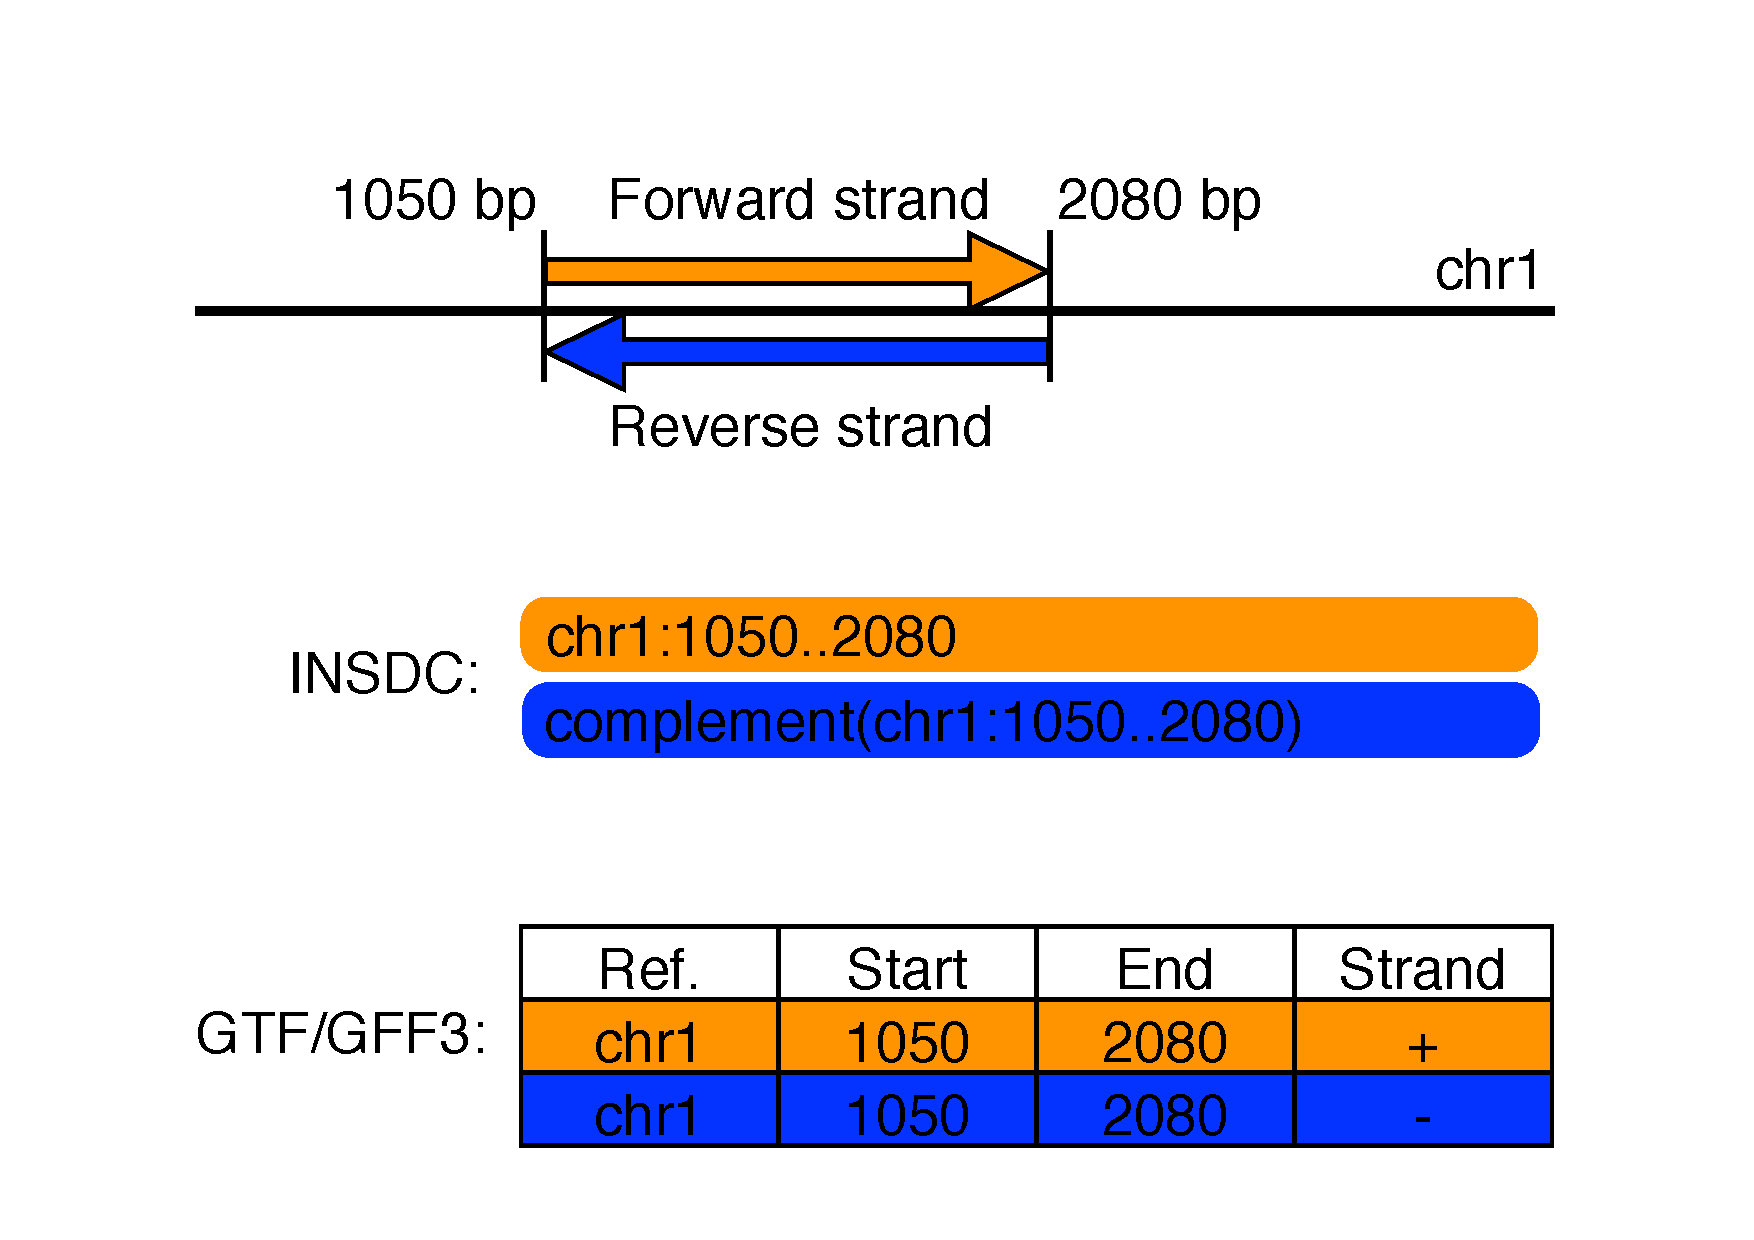
\includegraphics[width=10cm]{figures/figure-strand.pdf}
\end{center}
\caption{Assorted conventions for regions, start, end, and strands.
This figure shows two hypothetical features on a DNA sequence
(labelled \texttt{chr1}), on either the forward strand (orange) or
reverse strand (blue).
Using the INSDC location string notation, these regions are
``\texttt{1050..2080}'' and ``\texttt{complement(1050..2080)}''
respectively if implicitly given in terms of the reference chr1.
Using the GTF/GFF3 family of formats, regardless of the
strand these two locations are described with $start = 1050$
and $end = 2080$, and in general, $start \leq end$.
Biologically speaking, the start is strand dependent.
For the forward strand feature (orange), the start is 1050
while the reverse strand feature (blue) starts from 2080.
\textit{TODO - Replace with real example? Add FALDO illustration?}
}
\label{fig:strands}
\end{figure}
